% !TeX root = RJwrapper.tex
\title{Smooth Operator -- Modifying the Anhøj Rules to Improve Runs Analysis in
Statistical Process Control}
\author{by Jacob Anhøj, Tore Wentzel-Larsen}

\maketitle

\abstract{%
An abstract of less than 150 words.
}

% Any extra LaTeX you need in the preamble

\hypertarget{introduction}{%
\subsection{Introduction}\label{introduction}}

Within statistical process control (SPC) runs analysis is being used to
detect persistent shifts in process location over time.

Runs analysis deals with the natural limits of number of runs and run
lengths in random processes. A run is a series of one or more
consecutive elements of the same kind, for example heads and tails,
diseased and non-diseased individuals, or numbers above or below a
certain value. A run chart is a point-and-line chart showing data over
time with the median as reference line. In a random process, the data
points will be randomly distributed around the median, and the number
and lengths of runs will be predictable within limits. All things being
equal, if the process shifts, runs tend to become longer and fewer.
Consequently, runs analysis may help detect shifts in process location.
Process shifts are one form of non-random variation in time series data
that are of particular interest to quality control and improvement: If a
process shifts, it may be the result of planned improvement or unwanted
deterioration.

Several tests (or rules) based on the principles of runs analysis for
detection of shifts exist. In previous papers we demonstrated that the
currently best performing rules with respect to sensitivity and
specificity to shifts in process location are two simple tests
\citep{anhoej2014, anhoej2015, anhoej2018}:

\begin{itemize}
\item
  Shifts test: one or more unusually long runs of data points on the
  same side of the centre line.
\item
  Crossings test: the curve crosses the centre line unusually few times.
\end{itemize}

Collectively, we refer to these tests as the Anhøj rules. Critical
values for run length and number of crossings depend on the total number
of data points in the chart. The number of crossings follow a binomial
distribution, \(b(n - 1, 0.5)\), where n is the number of data points
and 0.5 the success probability. Thus, the lower prediction limit for
number of crossings may, for example, be set to the lower 5th percentile
of the corresponding cumulative binomial distribution \citep{chen2010}.
However, no closed form expression exists for the distribution of
longest runs. Consequently, the upper prediction limit for longest runs
has traditionally been either a fixed value (usually 7 or 8)
\citep{carey2002a} or an approximate value depending on n as with the
Anhøj rules: \(log_2(n) + 3\) rounded to the nearest integer
\citep{schilling2012}.

Using simulations, we have shown that runs analysis using the Anhøj
rules are comparable or even better at detecting minor to moderate
\emph{persistent} shift than the widely used Western Electric control
chart rules \citep{anhoej2018}.

Each of the two tests has an overall specificity (true negative
proportion) around 95\%. The sensitivity (true positive proportion) of a
test depends on the size of the shift (signal) relative to the random
variation inherent in the process (noise). When applied together, the
sensitivity increases, while the specificity decreases a bit.

\begin{figure}[htbp]
  \centering
  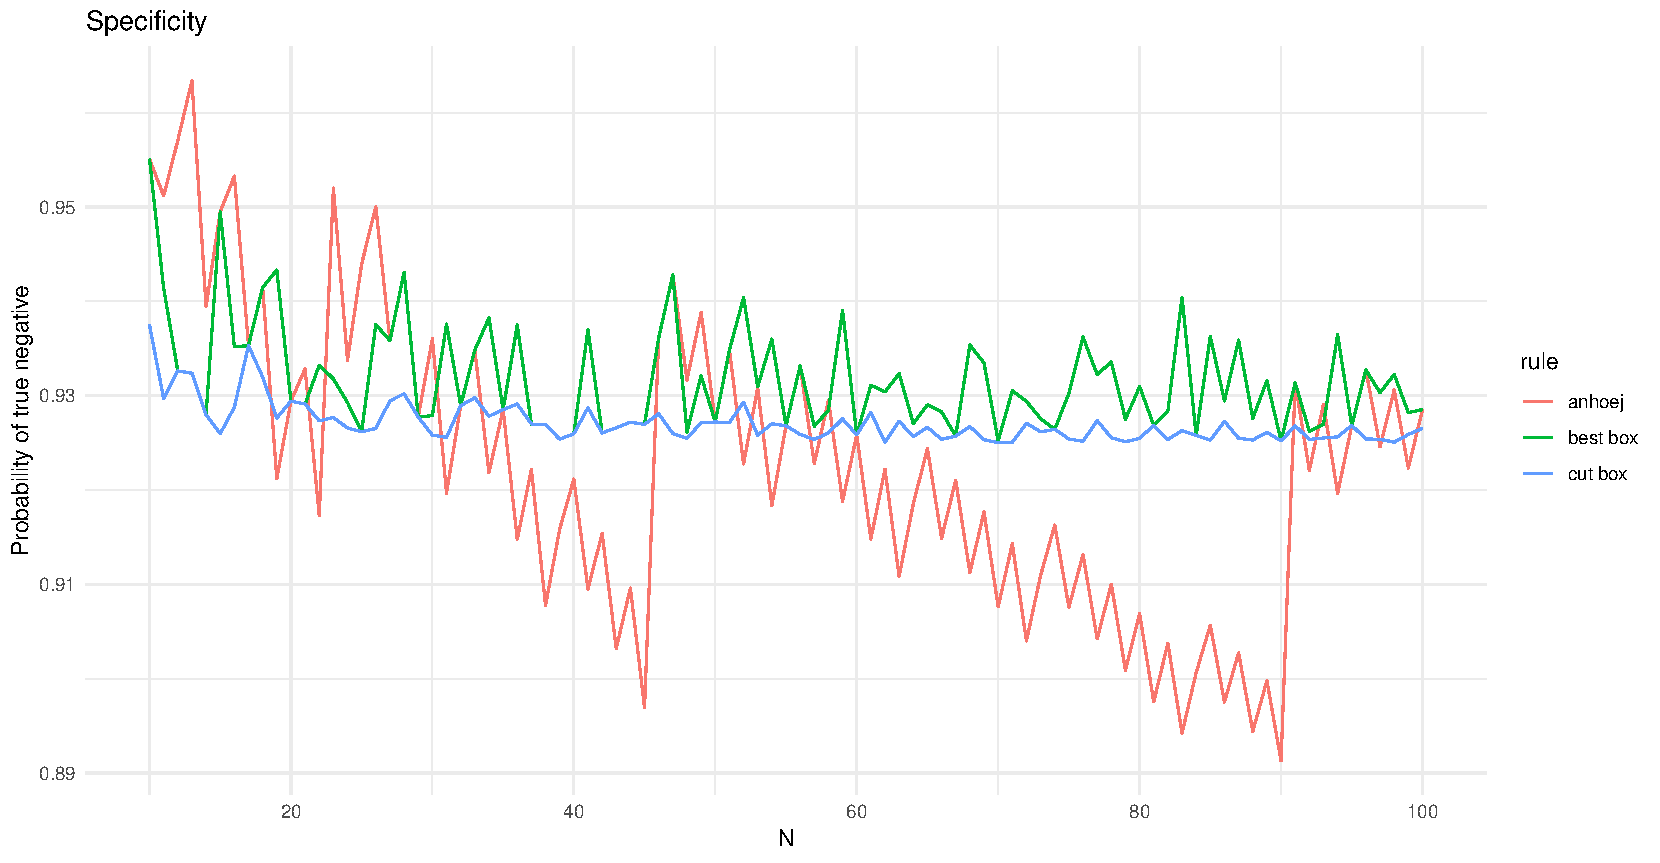
\includegraphics[width=\textwidth]{fig_spec.pdf}
  \caption{Specificity of the anhøj, best box, and cut box rules. N = number of data points in run chart. }
  \label{figure:spec}
\end{figure}

Historically, runs tests have mainly been studied in isolation as
individual tests. But what is really of interest -- because the rules
are linked, when one goes up, the other goes down -- is the properties
of the joint distribution of longest runs and number of crossings.

We recently released an R package, \CRANpkg{crossrun} \citep{twl2018},
that includes functions for calculating the joint probabilities of the
number of crossings (C) and longest runs (L) in random data series of
different lengths (N) and with and without shifts in process location
expressed in standard deviation units (SD). Figure \ref{figure:box11}
illustrates this for a run chart with N = 11 and SD = 0 (no shift). To
avoid very small numbers, the probabilities are shown using the times
representation, that is, the probabilities times \(2^{n-1}\), which is
1024 for N = 11. The red box encloses the combinations of C and L that
would indicate random variation according to the Anhøj rules (true
negatives). The area outside the box represents combinations of C and L
that would indicate non-random variation (false positives).

\begin{figure}[htbp]
  \centering
  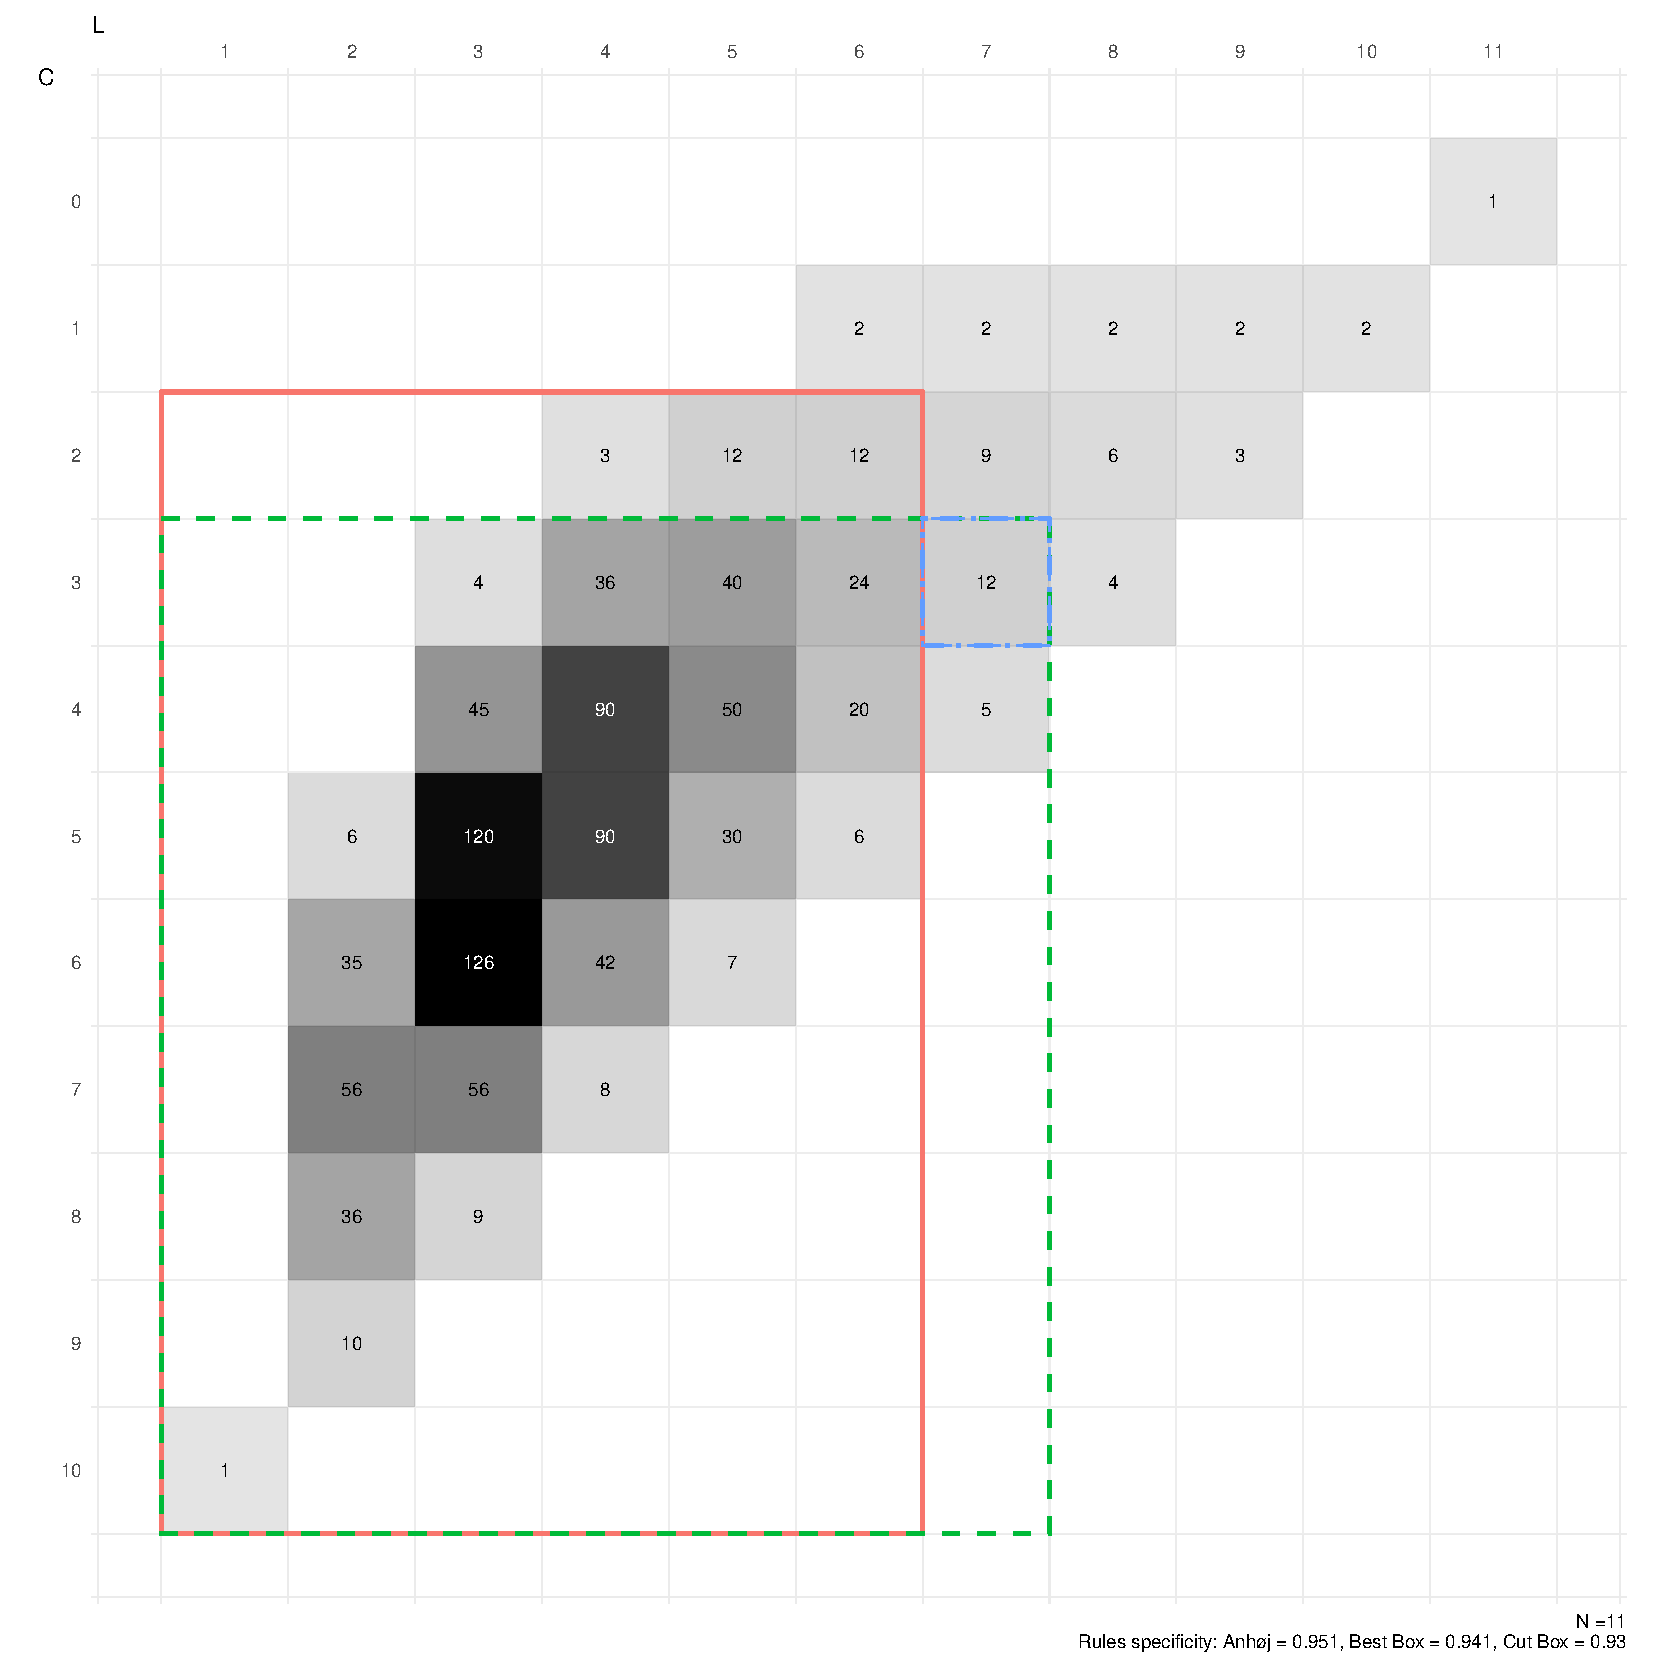
\includegraphics[width=0.8\textwidth]{fig_box11.pdf}
  \caption{Borders of the anhøj, best box, and cut box rules for N = 11 data points. 
           C = number of crossings, L = longest run.
           The numbers in the cells are times representation of of the joint
           probabilities of longest run and number of crossings.
           Anhøj = red solid, best box = green dashed, cut box = blue dot-dashed.}
  \label{figure:box11}
\end{figure}

With the \CRANpkg{crossrun} package it became feasible to calculate
exact joint probabilities of C and L for different N and SD. And
consequently, it became feasible to investigate the diagnostic
properties of run charts using exact values for specificity and
sensitivity rather than values based on time consuming and complicated
simulation studies.

As is clearly visible in Figure \ref{figure:spec} the specificity of the
Anhøj rules (red line) jumps up and down as N changes. This is a
consequence of the discrete nature of the two tests -- especially the
shifts test. Although the specificity of the Anhøj rules does not
decrease continuously as N increases as is the case with other rules, we
hypothesised that it would be possible to improve the diagnostic value
further by smoothing the specificity using minor adjustments to C and L
depending on N.

The aim of this study was to suggest a procedure for smoothing the
diagnostic properties of the Anhøj runs rules.

\hypertarget{methods}{%
\subsection{Methods}\label{methods}}

\hypertarget{likelihood-ratios-to-quantify-the-diagnostic-value-of-runs-rules}{%
\subsubsection{Likelihood ratios to quantify the diagnostic value of
runs
rules}\label{likelihood-ratios-to-quantify-the-diagnostic-value-of-runs-rules}}

The value of a diagnostic test is traditionally described using terms
like sensitivity and specificity. These parameters express the
probability of detecting the condition being tested for when it is
present and not detecting it when it is absent:

\[ \text{Specificity = P(no signal | no shift) = P(true negative}) \]
\[ \text{Sensitivity = P(signal | shift) = P(true positive}) \]

However, we usually seek to answer the opposite question: what is the
likelihood that a positive or negative test actually represents the
condition being tested for, which in our case is a shift in the
underlying process? Likelihood ratios (LR) do this:

\[ \text{LR+ = TP/FP = sensitivity/(1} - \text{specificity)} \]
\[ \text{LR- = FN/TN = (1} - \text{sensitivity)/specificity} \]

A likelihood ratio greater than 1 speaks in favour of the condition,
while a likelihood ratio less than 1 speaks against the condition. As a
rule of thumb, a positive likelihood ratio (LR+) greater than 10 is
considered strong evidence that the condition is present. A negative
likelihood ratio (LR-) smaller than 0.1 is considered strong evidence
against the condition \citep{deeks2004}. Thus, likelihood ratios are
useful measures of the diagnostic value of run charts
\citep{anhoej2015, anhoej2018}.

\hypertarget{best-box-and-cut-box-adjustments-to-improve-the-anhj-rules}{%
\subsubsection{Best box and cut box adjustments to improve the Anhøj
rules}\label{best-box-and-cut-box-adjustments-to-improve-the-anhj-rules}}

To fix some terms, we define a box as a square region
\(C \geq c, L \leq l\). These are the square regions that may be used to
define non-random variation. The corner of the box is its upper right
square \(C = c, L = l\). In Figure \ref{figure:box11} the box
\(C \geq 2, L \leq 6\), marked with red, specifies the Anhøj rules for
\(N=11\). The corner of this box is the square \(C = 2, L = 6\).

Based on the \CRANpkg{crossrun} package we developed two functions,
\code{bestbox()} and \code{cutbox()} that automatically seek to adjust
the critical values for C and L to balance between sensitivity and
specificity requirements. Specifically, the \code{bestbox()} function
finds the box with highest sensitivity for a pre-determined shift (the
target shift), among boxes with specificity \(\geq\) a pre-determined
value (the target sensitivity). The \code{cutbox()} function
subsequently cuts squares from the upper and right borders of the best
box, starting from the upper right corner while keeping specificity
\(\geq\) its target value, and the sensitivity for the target shift as
large as possible. The result of \code{cutbox()} is not necessarily a
box, but a reasonable region for declaring non-random variation with
only a few squares close to the corner possibly removed.

In this study we used a target specificity of 92.5\%, which is close to
the actual average specificity for the Anhøj rules for N = 10-100, while
the target shift was set at 0.8.

Figure \ref{figure:box11} illustrates these principles for a run chart
with 11 data points. Thus, for N = 11, the Anhøj rules would signal a
shift if C \textless{} 2 or L \textgreater{} 6; best box would signal if
C \textless{} 3 or L \textgreater{} 7; and cut box would signal if C
\textless{} 3 or L \textgreater{} 7 except when C = 3 and L = 7.

\hypertarget{results}{%
\subsection{Results}\label{results}}

We calculated the limits for the Anhøj, best box, and cut box rules
together with their corresponding positive test proportions and
log-likelihood ratios for N = 10-100 and SD = 0-3 (in 0.2 SD
increments). We stored the log of likelihood ratios to preserve
numerical precision. To get the actual likelihood values back, use
\code{exp(log-likelihood)}. The limits are presented in Table 1. The
full results set is available in the supplementary R data set
\file{cr\_bounds.rds}. The joint probabilities for N = 1-100 (using the
times representation) are provided in the \file{cr\_dist.rds} dataset.
To get the matric for, say, N = 11, use \code{cr\_dist[[11]]}. The R
code to produce the results and the figures in this article are
available in the supplementary materials \file{crossrunbox.R} and
\file{figs.R} respectively.

Figure \ref{figure:spec} illustrates the effect of the best box and cut
box procedures on the specificity of the runs analysis. As expected, the
variability in specificity with varying N is markedly reduced and kept
above and closer to the specified target -- more with cut box than with
best box.

Figure \ref{figure:pwr} shows the probabilities of getting a signal as a
function of N and SD. The upper left facet (SD = 0) contains the same
data as Figure \ref{figure:spec}. As expected and shown previously in
our simulations studies, the power of the runs analysis increases with
increasing N and SD. The smoothing effect of best box and cut box
appears to wear off as N and SD increases.

\begin{figure}[htbp]
  \centering
  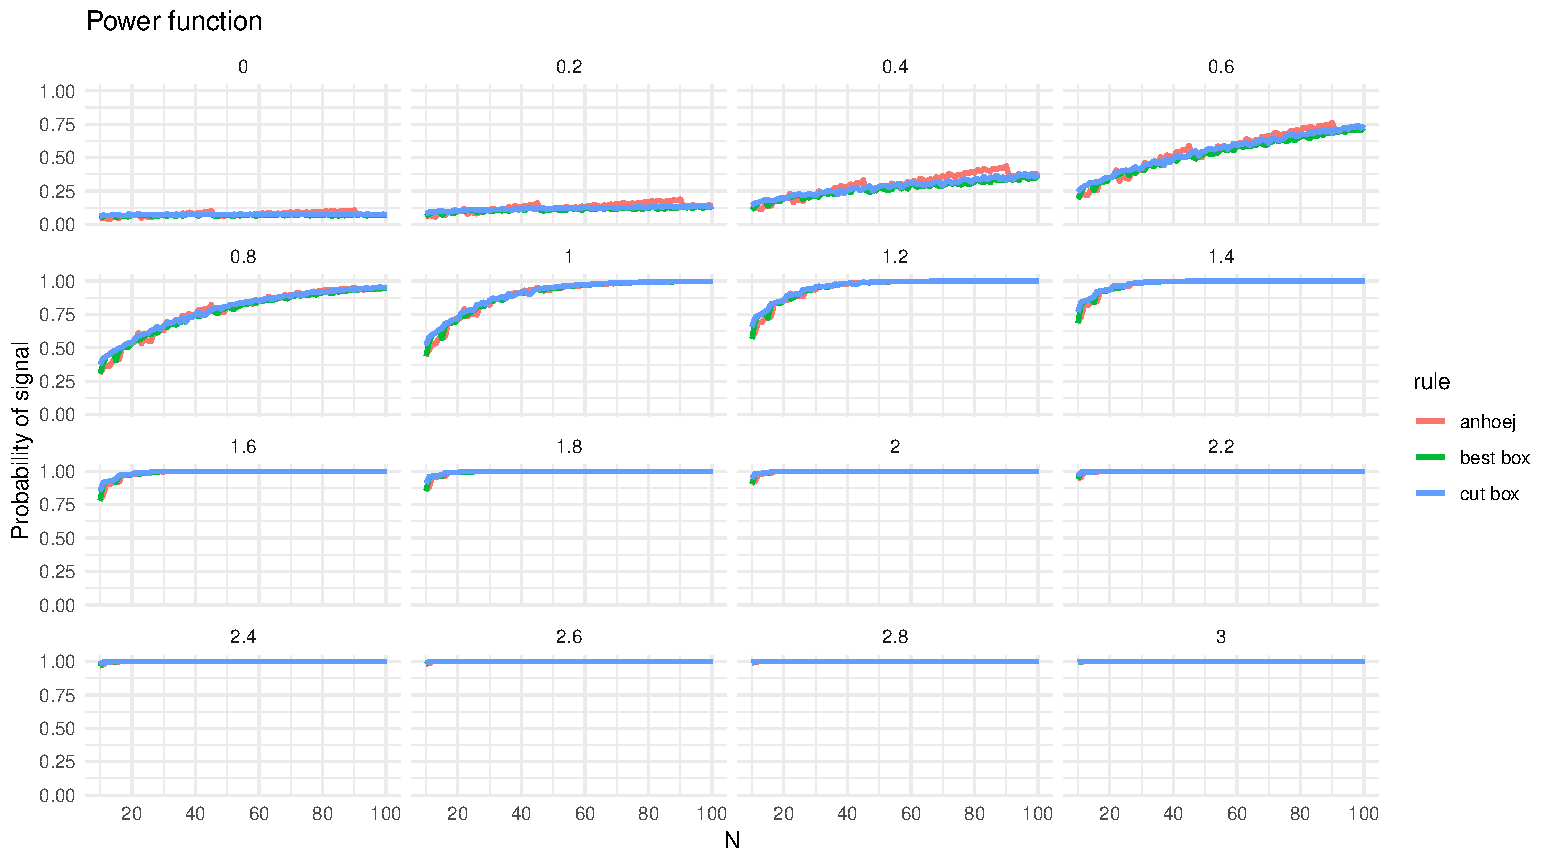
\includegraphics[width=\textwidth]{fig_pwr.pdf}
  \caption{Power function of Anhøj, best box, and cut box rules.
           N = number of data points in run chart.
           Numbers above each facet represent the size of the shift in standard
           deviation units (SD) that is present in data.}
  \label{figure:pwr}
\end{figure}

Figures \ref{figure:lrpos} and \ref{figure:lrneg} compare the positive
and negative likelihood ratios of the Anhøj rules to the box
adjustments. The smoothing effect appear to be of practical value only
for positive tests.

\begin{figure}[htbp]
  \centering
  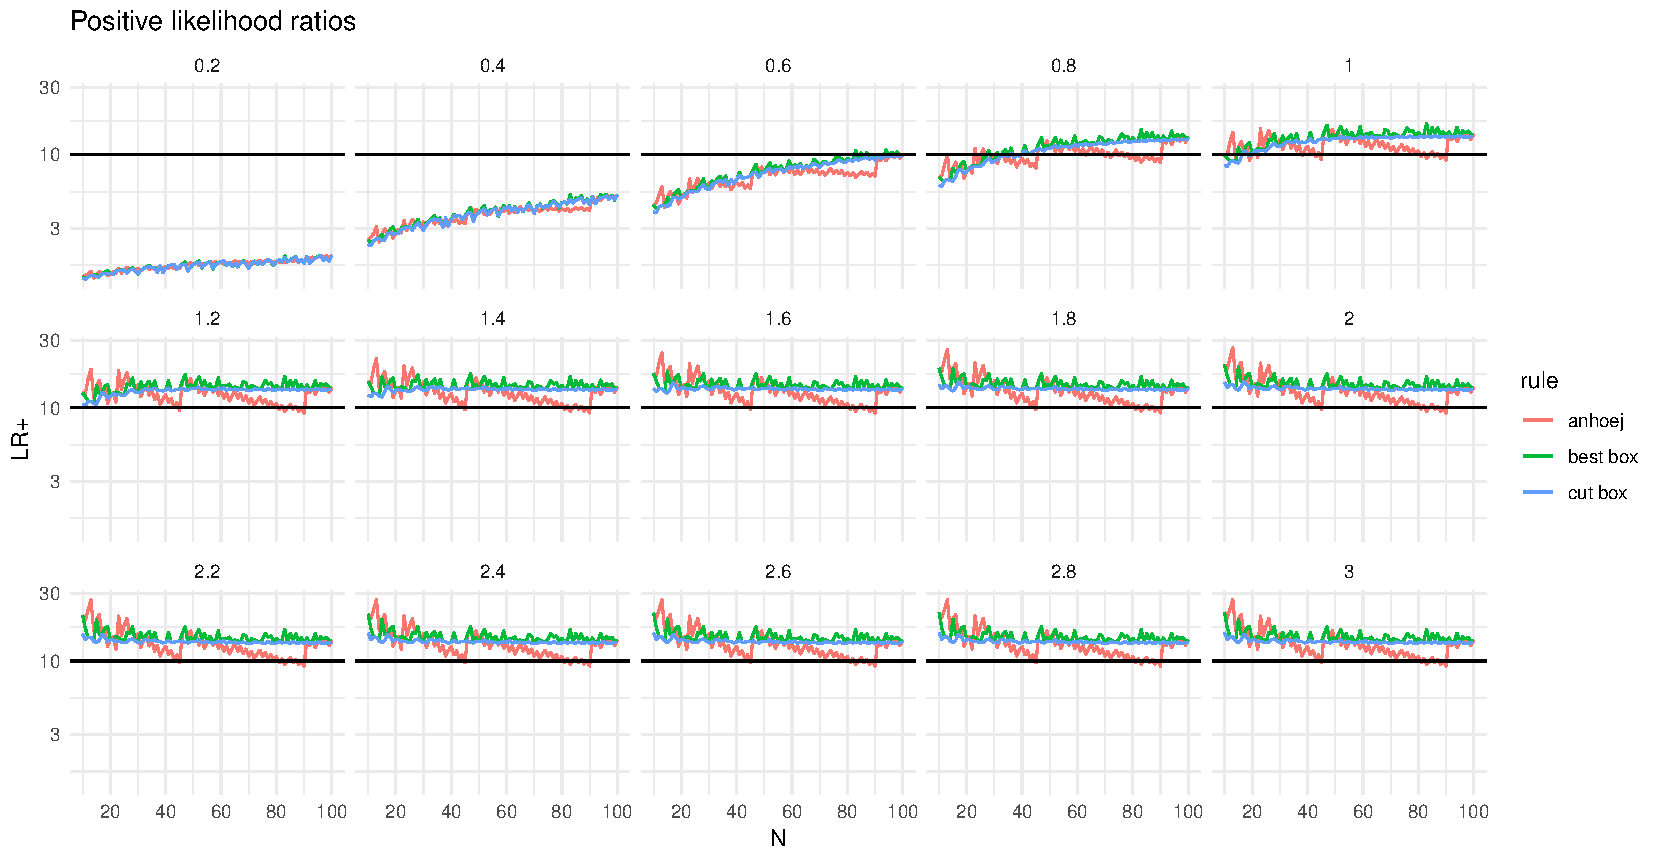
\includegraphics[width=\textwidth]{fig_lrpos.pdf}
  \caption{Positive likelihood ratio of Anhøj, best box, and cut box rules.
           N = number of data points in run chart.
           Numbers above each facet represent the size of the shift in standard
           deviation units that is present in data.}
  \label{figure:lrpos}
\end{figure}

\begin{figure}[htbp]
  \centering
  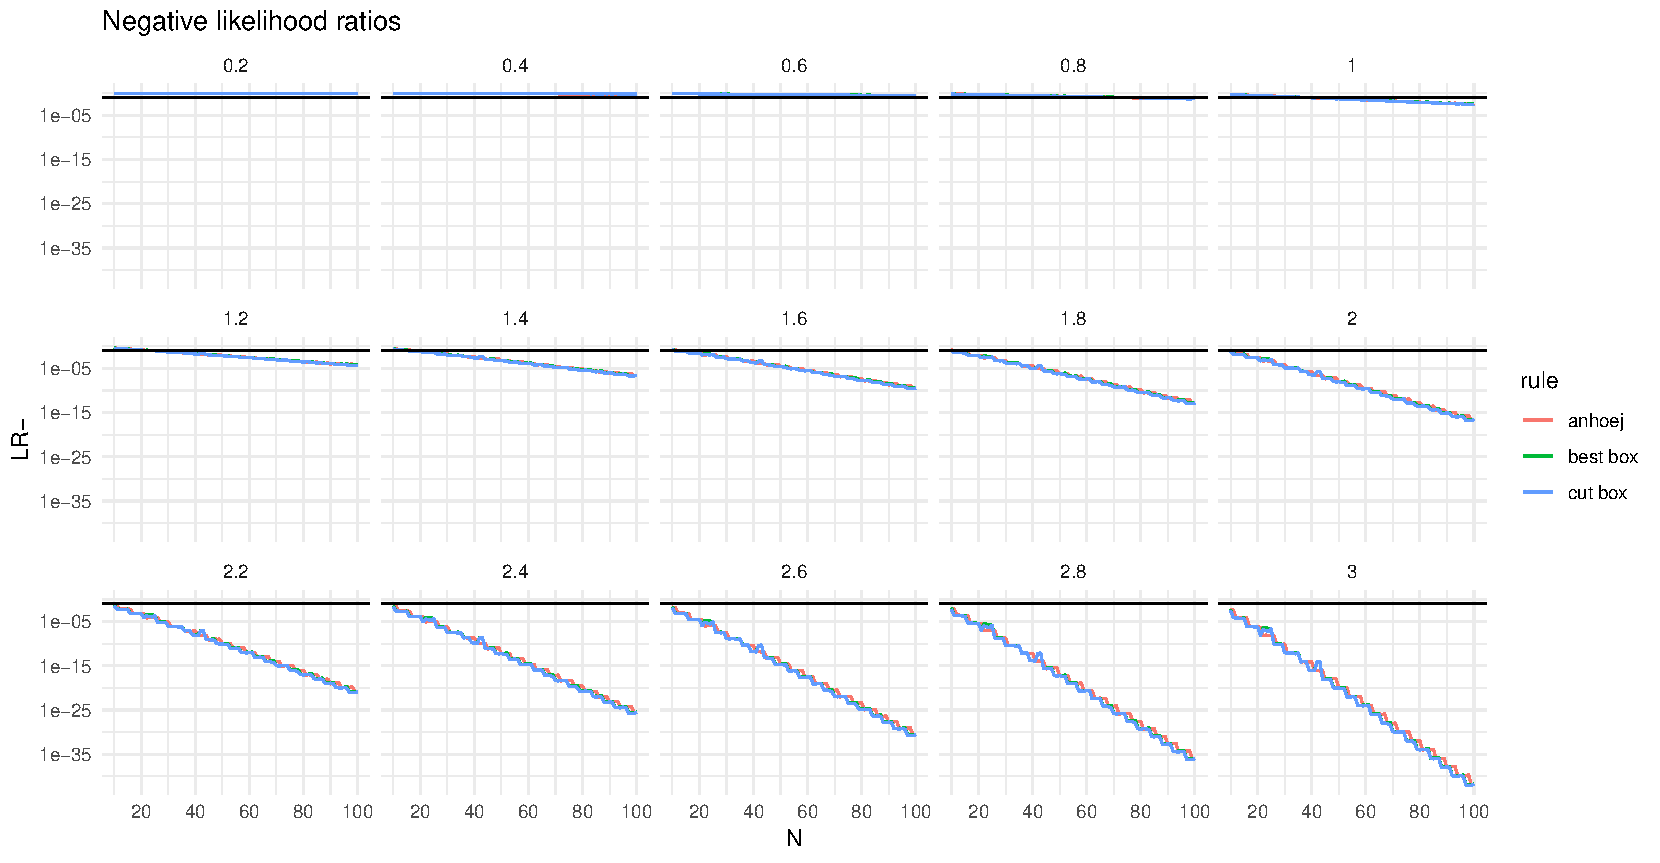
\includegraphics[width=\textwidth]{fig_lrneg.pdf}
  \caption{Negative likelihood ratio of Anhøj, best box, and cut box rules.
           N = number of data points in run chart.
           Numbers above each facet represent the size of the shift in standard
           deviation units (SD) that is present in data.}
  \label{figure:lrneg}
\end{figure}

\hypertarget{discussion}{%
\subsection{Discussion}\label{discussion}}

This study provided exact values for the diagnostic properties of the
Anhøj rules for run charts with 10-100 data points with and without
shifts up to 3 standard deviation units.

To our knowledge, and with the exeption of our own \CRANpkg{crossrun}
package, the properties of the joint distribution of number of crossings
and longest runs in random data series have not been studied before.

Furthermore, the study demonstrated that it is feasible to reduce the
variability in run chart specificity from varying number of data points
by using the best box and cut box adjustments of the Anhøj rules.

Most importantly, figures \ref{figure:lrpos} and \ref{figure:lrneg}
confirm, what we expected from years of practical experience using runs
analysis, that the Anhøj rules is a useful and robust method for
detection of persistent shifts only slightly larger than 1 standard
deviation units and with as little as 10-12 data points. Although, the
best box and cut box procedures will not change this, the box
adjustments may potentially improve the practical value of runs analysis
by reducing sudden shifts in sensitivity and specificity when the number
of available data points changes. However, this remains to be confirmed
in practice.

The study has tow important limitations. First, the calculations of box
probabilities require that the process centre, usually the median, is
fixed and known in advance, for example, from historical data. In
practice the centre line is often determined from the actual data in the
run chart, in which case the calculations of box probabilites do not
apply. Preliminary studies suggest that this is mostly relevant for
short data series. We plan to include a function in a future update of
\CRANpkg{crossrun} to calculate the box probabilites with emperical
centre lines.

Second, the procedures have so far only been checked for up to 100 data
points. Because of the iterative procedures and use of high precision
numbers (\CRANpkg{Rmpfr}) needed to calculate the joint distribution,
the computations are time consuming. On a laptop with an Intel Core i5
processor and 8 Gb RAM, it took about one hour (with all RAM consumed)
to complete \code{crossrunbox.R}. However, we have no reason to believe
that the procedures are not valid for N \textgreater{} 100, but the
application of the box procedures for larger N may be impractical at the
moment.

Also, one should be aware that the value of the box procedures rely on
the choice of target sensitivity and target shift values Other target
values may give very different diagnostic properties. However, by
supplying the R code, we encourage readers to adapt our findings to
their own needs.

As a note on the practical application of the box adjustment of the
Anhøj rules, we plan to include a \code{method} argument in the
\code{qic()} function of the \CRANpkg{qicharts2} package allowing the
user to choose between ``anhoej'', ``bestbox'', and ``cutbox'' methods
to identify non-random variation for up to 100 data points. For more
than 100 data points, the Anhøj rules will be applied.

\hypertarget{conclusion}{%
\subsection{Conclusion}\label{conclusion}}

\bibliography{RJreferences}

\hypertarget{appendix-bounds-table}{%
\subsection{Appendix: Bounds table}\label{appendix-bounds-table}}

\begin{Schunk}

\begin{longtable}{rrrrrrrrrr}
\caption{\label{tab:unnamed-chunk-1}Signal limits and specificity for the anhøj and best box rules and 
        borders for the cut box rules. N = number of trials. L = upper limit 
        for longest run, C = lower limit for number of crossings, Cbord and 
        Lbord = cut box borders to keep.}\\
\toprule
\multicolumn{1}{c}{ } & \multicolumn{2}{c}{Anhøj} & \multicolumn{2}{c}{Best box} & \multicolumn{2}{c}{Cut box} & \multicolumn{3}{c}{Specificity} \\
\cmidrule(l{3pt}r{3pt}){2-3} \cmidrule(l{3pt}r{3pt}){4-5} \cmidrule(l{3pt}r{3pt}){6-7} \cmidrule(l{3pt}r{3pt}){8-10}
N & L & C & L & C & Cbord & Lbord & Anhøj & Best box & Cut box\\
\midrule
\endfirsthead
\caption[]{Signal limits and specificity for the anhøj and best box rules a \textit{(continued)}}\\
\toprule
\multicolumn{1}{c}{ } & \multicolumn{2}{c}{Anhøj} & \multicolumn{2}{c}{Best box} & \multicolumn{2}{c}{Cut box} & \multicolumn{3}{c}{Specificity} \\
\cmidrule(l{3pt}r{3pt}){2-3} \cmidrule(l{3pt}r{3pt}){4-5} \cmidrule(l{3pt}r{3pt}){6-7} \cmidrule(l{3pt}r{3pt}){8-10}
N & L & C & L & C & Cbord & Lbord & Anhøj & Best box & Cut box\\
\midrule
\endhead
\
\endfoot
\bottomrule
\endlastfoot
10 & 2 & 6 & 2 & 6 & 3 & 5 & 0.9551 & 0.9551 & 0.9375\\
11 & 2 & 6 & 3 & 7 & 4 & 6 & 0.9512 & 0.9414 & 0.9297\\
12 & 3 & 7 & 3 & 6 &  &  & 0.9570 & 0.9326 & 0.9326\\
13 & 3 & 7 & 3 & 6 &  &  & 0.9634 & 0.9324 & 0.9324\\
14 & 4 & 7 & 3 & 6 &  &  & 0.9395 & 0.9280 & 0.9280\\
\addlinespace
15 & 4 & 7 & 4 & 7 & 6 & 6 & 0.9495 & 0.9495 & 0.9260\\
16 & 4 & 7 & 5 & 8 & 6 & 7 & 0.9533 & 0.9352 & 0.9288\\
17 & 5 & 7 & 5 & 7 &  &  & 0.9353 & 0.9353 & 0.9353\\
18 & 5 & 7 & 5 & 7 & 6 & 6 & 0.9415 & 0.9415 & 0.9320\\
19 & 6 & 7 & 5 & 7 & 6 & 5 & 0.9212 & 0.9433 & 0.9276\\
\addlinespace
20 & 6 & 7 & 6 & 7 &  &  & 0.9294 & 0.9294 & 0.9294\\
21 & 6 & 7 & 7 & 8 &  &  & 0.9328 & 0.9291 & 0.9291\\
22 & 7 & 7 & 6 & 7 & 7 & 6 & 0.9173 & 0.9332 & 0.9273\\
23 & 7 & 8 & 6 & 7 & 7 & 6 & 0.9520 & 0.9318 & 0.9277\\
24 & 8 & 8 & 6 & 7 & 7 & 6 & 0.9338 & 0.9293 & 0.9266\\
\addlinespace
25 & 8 & 8 & 6 & 7 &  &  & 0.9439 & 0.9262 & 0.9262\\
26 & 8 & 8 & 9 & 9 & 10 & 7 & 0.9500 & 0.9375 & 0.9265\\
27 & 9 & 8 & 9 & 8 & 10 & 7 & 0.9358 & 0.9358 & 0.9295\\
28 & 9 & 8 & 9 & 8 & 11 & 7 & 0.9431 & 0.9431 & 0.9302\\
29 & 10 & 8 & 10 & 8 &  &  & 0.9277 & 0.9277 & 0.9277\\
\addlinespace
30 & 10 & 8 & 11 & 10 & 12 & 9 & 0.9360 & 0.9279 & 0.9258\\
31 & 11 & 8 & 11 & 9 & 14 & 8 & 0.9197 & 0.9376 & 0.9256\\
32 & 11 & 8 & 11 & 8 &  &  & 0.9289 & 0.9289 & 0.9289\\
33 & 11 & 8 & 11 & 8 & 12 & 7 & 0.9348 & 0.9348 & 0.9298\\
34 & 12 & 8 & 11 & 8 & 13 & 7 & 0.9218 & 0.9382 & 0.9278\\
\addlinespace
35 & 12 & 8 & 12 & 8 &  &  & 0.9285 & 0.9285 & 0.9285\\
36 & 13 & 8 & 13 & 9 & 15 & 8 & 0.9148 & 0.9375 & 0.9291\\
37 & 13 & 8 & 14 & 10 &  &  & 0.9222 & 0.9270 & 0.9270\\
38 & 14 & 8 & 13 & 8 &  &  & 0.9078 & 0.9269 & 0.9269\\
39 & 14 & 8 & 15 & 11 &  &  & 0.9158 & 0.9254 & 0.9254\\
\addlinespace
40 & 14 & 8 & 15 & 9 &  &  & 0.9212 & 0.9260 & 0.9260\\
41 & 15 & 8 & 15 & 9 & 17 & 8 & 0.9095 & 0.9370 & 0.9287\\
42 & 15 & 8 & 14 & 8 &  &  & 0.9154 & 0.9260 & 0.9260\\
43 & 16 & 8 & 14 & 8 &  &  & 0.9032 & 0.9266 & 0.9266\\
44 & 16 & 8 & 17 & 10 &  &  & 0.9096 & 0.9272 & 0.9272\\
\addlinespace
45 & 17 & 8 & 17 & 9 &  &  & 0.8969 & 0.9270 & 0.9270\\
46 & 17 & 9 & 17 & 9 & 19 & 8 & 0.9361 & 0.9361 & 0.9281\\
47 & 17 & 9 & 17 & 9 & 20 & 7 & 0.9428 & 0.9428 & 0.9260\\
48 & 18 & 9 & 19 & 12 & 20 & 11 & 0.9317 & 0.9261 & 0.9255\\
49 & 18 & 9 & 19 & 10 & 21 & 9 & 0.9388 & 0.9321 & 0.9271\\
\addlinespace
50 & 19 & 9 & 19 & 9 &  &  & 0.9272 & 0.9272 & 0.9272\\
51 & 19 & 9 & 19 & 9 & 21 & 8 & 0.9348 & 0.9348 & 0.9271\\
52 & 20 & 9 & 19 & 9 & 21 & 7 & 0.9228 & 0.9404 & 0.9293\\
53 & 20 & 9 & 21 & 11 & 23 & 9 & 0.9308 & 0.9310 & 0.9258\\
54 & 21 & 9 & 21 & 10 & 23 & 8 & 0.9183 & 0.9360 & 0.9270\\
\addlinespace
55 & 21 & 9 & 21 & 9 &  &  & 0.9268 & 0.9268 & 0.9268\\
56 & 21 & 9 & 21 & 9 & 23 & 8 & 0.9331 & 0.9331 & 0.9259\\
57 & 22 & 9 & 23 & 12 & 25 & 11 & 0.9228 & 0.9268 & 0.9254\\
58 & 22 & 9 & 23 & 10 & 24 & 9 & 0.9295 & 0.9285 & 0.9260\\
59 & 23 & 9 & 23 & 10 & 26 & 8 & 0.9188 & 0.9390 & 0.9275\\
\addlinespace
60 & 23 & 9 & 23 & 9 &  &  & 0.9258 & 0.9258 & 0.9258\\
61 & 24 & 9 & 23 & 9 & 24 & 8 & 0.9148 & 0.9311 & 0.9282\\
62 & 24 & 9 & 25 & 11 & 27 & 9 & 0.9222 & 0.9304 & 0.9250\\
63 & 25 & 9 & 25 & 10 & 27 & 9 & 0.9108 & 0.9323 & 0.9273\\
64 & 25 & 9 & 26 & 11 & 27 & 10 & 0.9185 & 0.9270 & 0.9256\\
\addlinespace
65 & 25 & 9 & 26 & 10 & 27 & 9 & 0.9244 & 0.9290 & 0.9266\\
66 & 26 & 9 & 27 & 12 & 29 & 10 & 0.9149 & 0.9283 & 0.9254\\
67 & 26 & 9 & 27 & 10 &  &  & 0.9210 & 0.9257 & 0.9257\\
68 & 27 & 9 & 27 & 10 & 29 & 8 & 0.9112 & 0.9354 & 0.9267\\
69 & 27 & 9 & 28 & 11 & 29 & 8 & 0.9177 & 0.9335 & 0.9253\\
\addlinespace
70 & 28 & 9 & 29 & 14 & 30 & 13 & 0.9076 & 0.9252 & 0.9250\\
71 & 28 & 9 & 29 & 11 & 31 & 9 & 0.9143 & 0.9305 & 0.9251\\
72 & 29 & 9 & 29 & 10 & 30 & 9 & 0.9040 & 0.9294 & 0.9271\\
73 & 29 & 9 & 30 & 11 & 31 & 10 & 0.9109 & 0.9276 & 0.9262\\
74 & 29 & 9 & 30 & 10 &  &  & 0.9163 & 0.9264 & 0.9264\\
\addlinespace
75 & 30 & 9 & 31 & 12 & 32 & 9 & 0.9076 & 0.9302 & 0.9254\\
76 & 30 & 9 & 31 & 11 & 34 & 8 & 0.9132 & 0.9362 & 0.9252\\
77 & 31 & 9 & 31 & 10 & 33 & 9 & 0.9042 & 0.9322 & 0.9274\\
78 & 31 & 9 & 32 & 11 & 33 & 8 & 0.9100 & 0.9336 & 0.9255\\
79 & 32 & 9 & 33 & 13 & 37 & 11 & 0.9009 & 0.9275 & 0.9251\\
\addlinespace
80 & 32 & 9 & 33 & 11 & 35 & 9 & 0.9069 & 0.9310 & 0.9255\\
81 & 33 & 9 & 33 & 10 &  &  & 0.8975 & 0.9269 & 0.9269\\
82 & 33 & 9 & 34 & 11 & 36 & 10 & 0.9038 & 0.9284 & 0.9254\\
83 & 34 & 9 & 33 & 10 & 36 & 7 & 0.8942 & 0.9404 & 0.9263\\
84 & 34 & 9 & 35 & 11 &  &  & 0.9006 & 0.9258 & 0.9258\\
\addlinespace
85 & 34 & 9 & 35 & 11 & 38 & 8 & 0.9057 & 0.9363 & 0.9253\\
86 & 35 & 9 & 35 & 10 & 36 & 9 & 0.8975 & 0.9294 & 0.9273\\
87 & 35 & 9 & 35 & 10 & 38 & 8 & 0.9027 & 0.9359 & 0.9255\\
88 & 36 & 9 & 37 & 12 & 38 & 10 & 0.8944 & 0.9276 & 0.9253\\
89 & 36 & 9 & 37 & 11 & 39 & 9 & 0.8998 & 0.9316 & 0.9261\\
\addlinespace
90 & 37 & 9 & 38 & 12 &  &  & 0.8913 & 0.9252 & 0.9252\\
91 & 37 & 10 & 37 & 10 & 39 & 9 & 0.9314 & 0.9314 & 0.9268\\
92 & 38 & 10 & 39 & 13 & 41 & 12 & 0.9221 & 0.9262 & 0.9254\\
93 & 38 & 10 & 39 & 11 & 40 & 10 & 0.9291 & 0.9270 & 0.9255\\
94 & 39 & 10 & 39 & 11 & 42 & 8 & 0.9196 & 0.9365 & 0.9256\\
\addlinespace
95 & 39 & 10 & 39 & 10 &  &  & 0.9268 & 0.9268 & 0.9268\\
96 & 39 & 10 & 39 & 10 & 41 & 8 & 0.9327 & 0.9327 & 0.9254\\
97 & 40 & 10 & 41 & 12 & 42 & 9 & 0.9246 & 0.9303 & 0.9254\\
98 & 40 & 10 & 41 & 11 & 44 & 9 & 0.9306 & 0.9322 & 0.9251\\
99 & 41 & 10 & 42 & 12 & 43 & 10 & 0.9223 & 0.9282 & 0.9259\\
\addlinespace
100 & 41 & 10 & 41 & 10 & 42 & 9 & 0.9285 & 0.9285 & 0.9265\\*
\end{longtable}

\end{Schunk}


\address{%
Jacob Anhøj\\
Rigshospitalet, University of Copenhagen\\
Denmark\\
}
\href{mailto:jacob@anhoej.net}{\nolinkurl{jacob@anhoej.net}}

\address{%
Tore Wentzel-Larsen\\
Centre for Child and Adolescent Mental Health, Eastern and Southern
Norway \& Centre for Violence and Traumatic Stress Studies, Oslo, Norway\\
Norway\\
}
\href{mailto:tore.wentzellarsen@gmail.com}{\nolinkurl{tore.wentzellarsen@gmail.com}}

